\section{Limites et continuité}
\activity{Rappels sur les limites}{1}{
 Désemparé  par les  résultats  des deux devins, Dansou décide de se consacrer à ses études pour réussir à son examen. Cependant, il a quelques difficultés dans le calcul des limites. Tu vas l'aider en te basant sur tes connaissances antérieurs, pour résoudre les consigne de cette séquence.
}
\subsection{Limites de fonctions usuelles}
Soit $k\in \R$, et $n$ un entier naturel non nul.
\begin{boite}
	\begin{multicols}{2}
		\item[$\bullet$] \limite{x}{-\infty}{k=k} et \limite{x}{+\infty}{k=k}
		\item[$\bullet$] \limite{x}{+\infty}{\sqrt{x}=+\infty}
		\item[$\bullet$] \limite{x}{+\infty}{x^n=+\infty}
		\item[$\bullet$] \limite{x}{-\infty}{x^n =
			\begin{cases}
				+\infty \text{, si }n\text{ est pair.}\\
				-\infty\text{, si }n\text{ est impair.}
			\end{cases}
		}
		\item[$\bullet$] \limite{x}{-\infty }{\f{1}{x^n}=0} et  \limite{x}{+\infty }{\f{1}{x^n}=0}
		\item[$\bullet$] \limite{x}{0}{\f{\sin x}{x}=1}\\ \item[$\bullet$]\limite{x}{0}{\f{\tan x}{x}=1}\\
		\item[$\bullet$] \limite{x}{0}{\f{\cos x -1}{x}=0}\\
		\item[$\bullet$] \limite{x}{0}{\f{1-\cos x}{x^2}=\f{1}{2}}
	\end{multicols}
\end{boite}
\subsection{Opérations algébriques}
Soient $f$ et $g$ deux fonctions numériques telles que $D_f\cap D_g\neq \emptyset$. $x_0$ est un réel, ou égal à $-\infty$, ou à $+\infty$, au voisinage duquel $f$ et $g$ sont définies.
{\newcolumntype{Y}{>{\raggedleft\arraybackslash}X}% see tabularx
	\tcbset{enhanced,fonttitle=\bfseries\large,
		colback=yellow!10!white,colframe=red!50!black,colbacktitle=green!30!white,
		coltitle=black,center title}
	\begin{tcolorbox}[tabularx={p{2.3cm}|p{1.8cm}||p{0.7cm}||p{3cm}|p{3cm}|X},title=Opérations sur les limites,sharp corners]
		Si \limite{x}{x_0}{f(x)=} & \limite{x}{x_0}{g(x)=}	& alors	& \limite{x}{x_0}{\big(f+g\big)(x)=}	& 	\limite{x}{x_0}{\big(f\times g\big)(x)=}& \limite{x}{x_0}{\bigg(\f{f}{g}\bigg)(x)=}\\\hline\hline
		\centering$\ell$	& \centering$\ell '$ &  &\centering $\ell +\ell '$& \centering$\ell\times \ell'$ &$\begin{cases}
		\f{\ell}{\ell'}\text{; si }\ell\neq 0\text{ et }\ell'\neq 0\\
		0\text{; si }\ell=0\text{ et }\ell'\neq 0\\
		\pm\infty\text{; si }\ell \neq 0\text{, }\ell'=0^\pm
		\end{cases}$\\\hline
		\centering$0$&\centering$0$&&\centering$0$&\centering$0$&\textbf{On ne peut pas conclure}\\\hline
		\centering$\ell \neq 0$&\centering$\pm\infty$&&\centering$\pm\infty$&$\begin{cases}
		\pm\infty\text{; si }l>0\\
		\mp\infty\text{; si }l<0
		\end{cases}$&$0$\\\hline
		\centering$0$&\centering$\pm\infty$& &\centering$\pm\infty$&\textbf{On ne peut pas conclure}&$0$\\\hline
		
		\centering$\pm\infty$&\centering$\ell'\neq 0$& &\centering$\pm\infty$&$\begin{cases}
		\pm\infty\text{; si }\ell'>0\\
		\mp\infty\text{; si }\ell'<0
		\end{cases}$&$\begin{cases}
		\pm\infty\text{; si }\ell'>0\\
		\mp\infty\text{; si }\ell'<0
		\end{cases}$\\\hline
		\centering$\pm\infty$&\centering$ 0$& &\centering$\pm\infty$&\textbf{On ne peut pas conclure}&$\begin{cases}
		\pm\infty\text{; si }0^\pm\\
		\pm\infty\text{; si }0^\pm
		\end{cases}$\\\hline
		\centering$\pm\infty$&\centering$\pm\infty$& &\centering$\pm\infty$&\centering$+\infty$&\textbf{On ne peut pas conclure}\\\hline
		\centering$\pm\infty$&\centering$\mp\infty$& &\textbf{On ne peut pas conclure}&\centering$-\infty$&\textbf{On ne peut pas conclure}\\\hline
\end{tcolorbox}}
%\begin{remarque}
%\subsection{Formes indéterminées}
Les cas où on ne peut pas conclure sont les formes indéterminées. Ceux sont les cas : \og $-\infty+(+\infty)$\fg{ }; \og $0\times \infty$\fg{ }; \og $\f{0}{0}$\fg{ } et \og $\f{\infty}{\infty}$\fg{ }. Ils nécessitent des transformations appropriées (factorisation, expression conjuguée, division euclidienne \dots)
\begin{remark}
	\begin{itemize}
		\item[\ding{182}] La limite en l'infini d'une fonction polynôme est égale à la limite de son monôme de plus haut degré.
		\item[\ding{183}] La limite à l’infini d’une fonction rationnelle est égale à la limite à l’infini du
		quotient simplifié de ses termes de plus hauts degrés.
	\end{itemize}
\end{remark}
\vspace*{-0.5cm}
\begin{center}
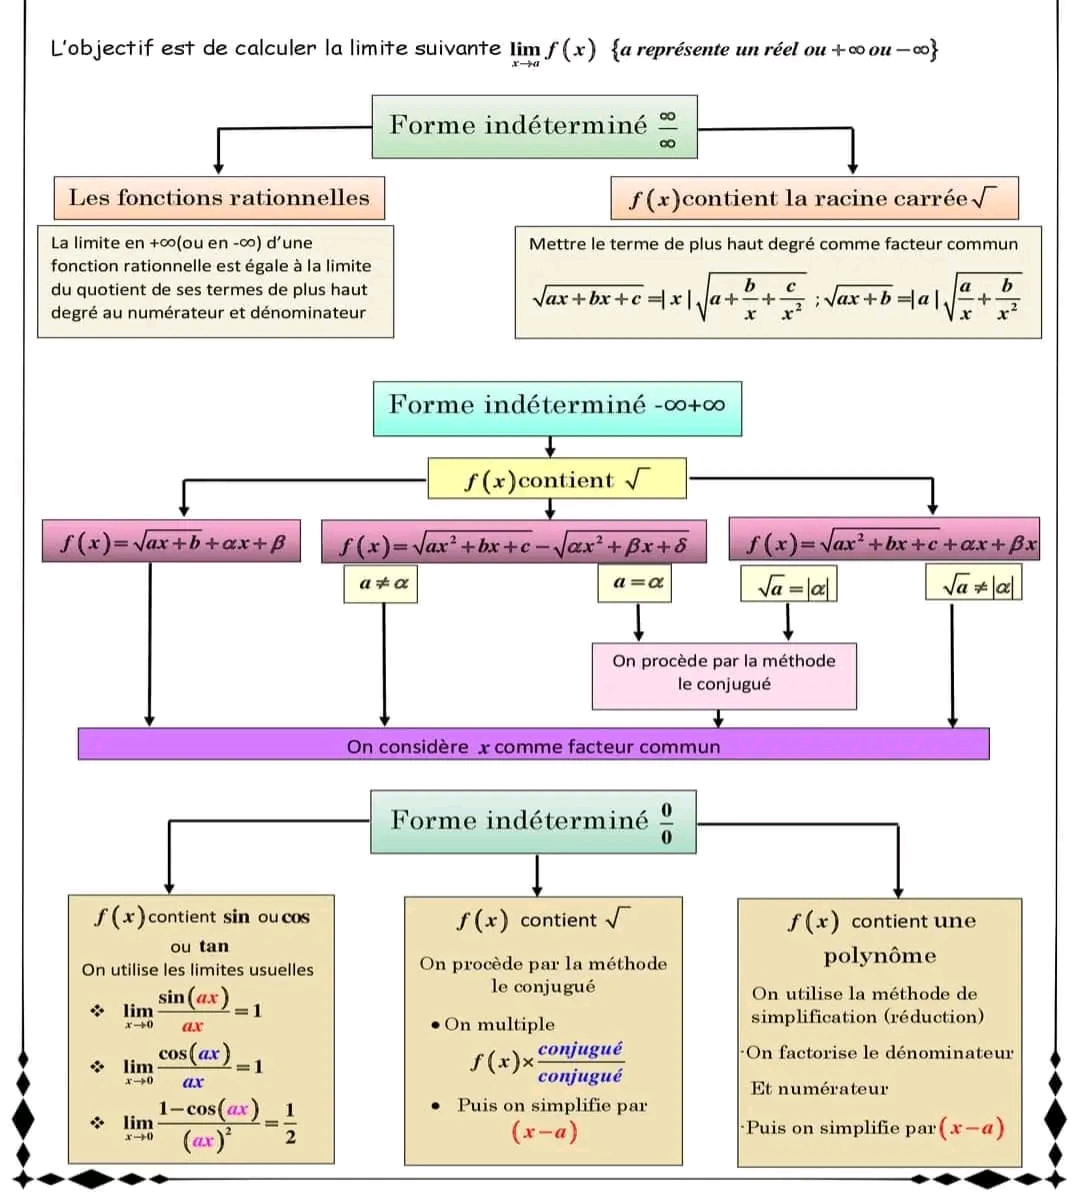
\includegraphics[scale=0.45]{images/forme_ind}
\end{center}
\vspace*{-0.5cm}
\consigne{Consolidation}{1.1}{
\be \item Calcule les limites en $-\infty$ ; $+\infty$ et en $-1$ de la fonction $f$ dans chacun des cas ci-dessous :
\begin{tasks}(3)
\task $f(x)=-2x^3-7x^2+3x-1$
\task $f(x)=\F{3x^2-5x+11}{2x^2+3x-7}$
\task $f(x)=\F{2x-6}{x^2-2x-3}$.
\end{tasks}
\item Calcule les limites suivantes :
\begin{tasks}(3)
	\task \limite{x}{0}{\bigg(\f{\sqrt{9+x}}{x}\bigg)}
	\task \limite{x}{0}{\bigg(\f{1-\cos^2 x}{5x}\bigg)}
	\task \limite{x}{1}{\bigg(\f{\sqrt{3x+2}-\sqrt{11x-6}}{x-\sqrt{3+x}+1}\bigg)}
\end{tasks}
	\item Calcule les limites en $+\infty$ et en $-\infty$ de la fonction $f$ dans chacun des cas ci-dessous :
	\begin{tasks}(3)
		\task $f(x)=\sqrt{x^2+1}+x-2$
		\task $f(x)=\sqrt{2x^2-x+1}+2x+3$
	\end{tasks}
\ee
}
  \subsection{Théorèmes de comparaison}
 % \vspace*{-0.5cm}
\begin{propriete}[s]
	Soit $a$, un nombre réel ou égal à $+\infty$ ou $-\infty$. $\ell$ et $\ell'$, deux nombres réels. $f$, $g$ et $h$ sont trois fonctions.
	\begin{itemize}
		\item Si $\begin{cases}
		\limite{x}{a}{f(x)=\ell} \\
		\limite{x}{a}{g(x)=\ell'}\\
		f(x)\leq g(x)  
		\end{cases}\implies \ell \leq \ell'$
		\item Si $\begin{cases}
		g(x)\leq f(x)\\
		\limite{x}{a}{g(x)=+\infty}
		\end{cases}\implies \limite{x}{a}{f(x)=+\infty} $
		\item Si $\begin{cases}
		f(x)\leq g(x)\\
		\limite{x}{a}{g(x)=-\infty}
		\end{cases}\implies \limite{x}{a}{f(x)=-\infty} $
		\item Si $\begin{cases}
		f(x)\leq g(x)\leq h(x)\\
		\limite{x}{a}{f(x)=\limite{x}{a}{h(x)=\ell}}
		\end{cases}\implies \limite{x}{a}{g(x)=\ell} $
		\par En particulier, si \limite{x}{a}{f(x)=\ell} et $\forall x \in I\setminus\{a\}$, $a\leq f(x)\leq b$, alors $\ell\in \intervFF{a}{b}$
		\item Si $\begin{cases}
		\lvert f(x)-l\rvert \leq g(x)\\
		\limite{x}{a}{g(x)=0}
		\end{cases}\implies \limite{x}{a}{f(x)=\ell}$
	\end{itemize}
Les résultats des propriétés précédentes sont valables pour les cas de limites à gauche et à droite en $a$.
\end{propriete}
\consigne{Utilisation des propriétés de comparaison}{1.2}{
\be \item Soit $f$ et $g$ deux fonctions définies sur \intervOO{0}{+\infty}
par $f(x)=1-\f{1}{x}$ et $g(x)=2-\f{1}{x}$.
\be \item Compare $f$ et $g$ sur \intervOO{0}{+\infty}.
\item Compare les limites de $f$ et $g$, quand $x$ tend vers $+\infty$.\ee
\item Soit $f$ : $x\longmapsto \sqrt{2x^2+x}$.
\be \item Démontre que pour tout $x\geq 0$, $f(x)>x$.
\item Déduis-en \limite{x}{+\infty}{f(x)}.\ee
\item Soit $g$ : $x\longmapsto \f{x+\sin x}{2x+1}$.
\be \item Démontre que pour tout $x\geq 0$ ; $\f{x-1}{2x+1}\leq g(x)\leq \f{x+1}{2x+1}$.
\item Déduis-en \limite{x}{+\infty}{g(x)}.\ee
\item Soit $h$ : $x\longmapsto \f{4\sin x+3x}{x-1}$.
 \be \item Vérifie que pour tout $x>1$, $h(x)=\f{4\sin x+3}{x-1}+3$.
\item Montre que pour tout $x>1$, $\big\lvert h(x)-3\big\rvert\leq \f{7}{x-1}$.
\item Déduis-en \limite{x}{+\infty}{\big(h(x)-3\big)}, puis \limite{x}{+\infty}{h(x)}.\ee\ee
}
\consigne{Limite d'une fonction composée}{1.3}{
Soit $u$, la fonction définie par $u(x)=\sqrt{\f{2x-1}{x-1}}$.
\be \item Calcule \limite{x}{+\infty}{u(x)}.
\item \be \item Écris $u$ comme composée de deux fonctions $f$ et $g$ où, $f$ est une fonction de référence et $g$ est une fonction rationnelle.
\item Calcule \limite{x}{+\infty}{g(x)}, \limite{x}{b}{f(x)}, avec $b=\limite{x}{+\infty}{g(x)}$.
\item Que remarques-tu ? Comment peut-on calculer la limite d'une fonction composée $f\circ g$ ?\ee\ee
}
\subsection{Limite d'une fonction composée}
Chacune des lettres $a$, $b$ et $c$ désigne soit un réel, soit $+\infty$, soit $-\infty$.\\
\begin{propriete}
	$f$ et $g$ sont deux fonctions numériques. $a$ un élément ou une borne d’un intervalle sur lequel $g\circ f$ est
	définie.
	\par Si \limite{x}{a}{f(x)=b} et \limite{x}{b}{g(x)=c}, alors \limite{x}{a}{\big(g\circ f\big)(x)=c}	
\end{propriete}
\par Les résultats de la propriété précédente sont valables pour les cas de limites à gauche et à droite en $a$.
 \subsection{Limite d'une fonction monotone sur un intervalle ouvert}
\subsubsection{Limite d'une fonction croissante sur un intervalle ouvert}
\begin{propriete}
	Soit $f$, une fonction croissante sur un intervalle \intervOO{a}{b}, $(a\in \R$, $b\in \R$ et $a<b$).
	\begin{itemize}
		\item[$\bullet$] Si $f$ est majorée sur \intervOO{a}{b}, alors $f$ admet une limite finie à gauche en $b$.
		\item[$\bullet$] Si $f$ n'est pas majorée sur \intervOO{a}{b}, alors \limite{x}{b\\x<b}{f(x)=+\infty}.
		\item[$\bullet$] Si $f$ est minorée sur \intervOO{a}{b}, alors $f$ admet une limite finie à droite en $a$.
		\item[$\bullet$] Si $f$ n'est pas minorée sur \intervOO{a}{b}, alors \limite{x}{a\\x>a}{f(x)=-\infty}.
	\end{itemize}
\end{propriete}
\subsubsection{Limite d'une fonction décroissante sur un intervalle ouvert}\vspace*{-0.3cm}
\begin{propriete}
	Soit $f$, une fonction décroissante sur un intervalle \intervOO{a}{b}, $(a\in \R$, $b\in \R$ et $a<b$).
	\begin{itemize}
		\item[$\bullet$] Si $f$ est minorée sur \intervOO{a}{b}, alors $f$ admet une limite finie à gauche en $b$.
		\item[$\bullet$] Si $f$ n'est pas minorée sur \intervOO{a}{b}, alors \limite{x}{b\\x<b}{f(x)=-\infty}.
		\item[$\bullet$] Si $f$ est majorée sur \intervOO{a}{b}, alors $f$ admet une limite finie à droite en $a$.
		\item[$\bullet$] Si $f$ n'est pas majorée sur \intervOO{a}{b}, alors \limite{x}{a\\x>a}{f(x)=+\infty}.
	\end{itemize}
\end{propriete}
%\activity{Continuité}{2}{
%}
\subsection{Application du calcul des limites : étude des branches infinies}
$f$ désigne une fonction d'ensemble de définition $D_f$ et $(\mathcal{C}_f)$ sa courbe représentative.
\par On dit que $(\mathcal{C}_f)$ admet une branche infinie dans les cas suivant :
\begin{itemize}
\item en $+\infty$ ou en $-\infty$, $f$ a une limite finie ou infinie.
\item en $x_0$, $f$ a une limite infinie.
\end{itemize}%\vspace*{-0.3cm}
\begin{center}
	\textbf{\textsf{\uline{Organigramme d'étude d'une branche infinie.}}}
\end{center}
\tikzset{ midd/.style={
		decoration={
			markings,
			mark=at position 0.5 with {%
				\makebox[6pt][l]{\arrow{triangle 45}},
			},
		},
		postaction={decorate},{Circle[]}-{Circle[]}
	},}%
\begin{tikzpicture}[yscale=2,xscale=1,rounded corners=4pt]
	% xscale et yscale permettent d'ajuster largeur et hauteur
	% positionner les nœuds
	\node(a) at (-3,0)[rectangle,draw,,text width=2.5 cm,fill=blue!30,text centered] {$\lim\limits_{x \to \infty} f(x)=b$};
	\node(b) at (6,0)[rectangle,draw,,text width=2.7 cm,fill=blue!30,text centered] {$\lim\limits_{x \to \infty} f(x)=\infty$};
	\node(c) at (12.2,0)[rectangle,draw,,text width=2.5 cm,fill=blue!30,text centered] {$\lim\limits_{x \to x_0} f(x)=\infty$};
	%
	\node(d) [below left=2cm of b ,rectangle,draw,text width=4.5cm,text centered] {$\lim\limits_{x \to \infty} \big[f(x)-(ax+b)\big]=0$};
	\node(e) [right=0.2cm of d ,rectangle,draw,text width=3.4cm,text centered] {$\lim\limits_{x \to \infty} \dfrac{f(x)}{x}=a$ ($a\neq 0$)};
	\node(f) [right=0.2cm of e ,rectangle,draw,text width=2.5cm,text centered] {$\lim\limits_{x \to \infty} \dfrac{f(x)}{x}=\infty$};
	\node(g) [right=0.2cm of f ,rectangle,draw,text width=2.5cm,text centered] {$\lim\limits_{x \to \infty} \dfrac{f(x)}{x}=0$};
	%
	\node(h) [below =1.7cm of d ,rectangle,draw,text width=3.8cm,text centered,xshift=1.9cm] {$\lim\limits_{x \to \infty} \big[f(x)-(ax)\big]=b$};
	\node(i) [right=0.3cm of h,rectangle,draw,text width=4.1cm,text centered] {$\lim\limits_{x \to \infty} \big[f(x)-(ax)\big]=\infty$};
	%
	\node(j) [below left=3.5cm of h ,rectangle,draw,text width=2.5cm,text centered,xshift=0cm] {$(\mathcal{C}_f)$ admet une asymptote (horizontale) d'équation $y=b$ au voisinage de $\infty$};
	\node(k) [right=0.3cm of j ,rectangle,draw,text width=2.5cm,text centered] {La droite d'équation $y=ax+b$ est une asymptote (oblique) de $(\mathcal{C}_f)$ au voisinage de $\infty$};
	\node(l) [right=0.3cm of k ,rectangle,draw,text width=2.5cm,text centered] {$(\mathcal{C}_f)$ admet une branche parabolique de direction la droite d'équation $y=ax$ au voisinage de $\infty$};
	\node(m) [right=0.3cm of l ,rectangle,draw,text width=2.5cm,text centered] {$(\mathcal{C}_f)$ admet une branche parabolique de direction l'axe des ordonnées au voisinage de $\infty$};
	\node(n) [right=0.3cm of m ,rectangle,draw,text width=2.5cm,text centered] {$(\mathcal{C}_f)$ admet une branche parabolique de direction l'axe des abscisses au voisinage de $\infty$};
	\node(o) [right=0.3cm of n ,rectangle,draw,text width=2cm,text centered] {$(\mathcal{C}_f)$ admet une asymptote (verticale) d'équation $x=x_0$};
	%%%arrow%%%%%%%%%%%%%%%%%%%
	%%%%%%%%%%%%%%%%%%
	\draw[midd]([xshift=-0.3cm]a.south)--(j.north);
	%\draw[midd]([xshift=-0.5cm]d.west)|-(k.west);
	\draw[midd]([xshift=0.65cm]d.south west)--([xshift=0.6cm]k.north west);
	\draw[midd](b)-|([xshift=2.5cm]d);
	\draw[midd](b.south)--([yshift=-0.1cm]b.south)-|([xshift=0.7cm]e.north west);
	\draw[midd ](b.south)--([yshift=-0.1cm]b.south)-|(f.north);
	\draw[midd](b.east)--([xshift=1cm]b.east)-|([xshift=-1cm]g.north);
	%
	\draw[midd](e.south)--([yshift=-0.15cm]e.south)-|(h.north);
	\draw[midd](e.south)--([yshift=-0.15cm]e.south)-|(i.north);
	\draw[midd]([xshift=-0.1cm]f.south)--([yshift=-0.2cm]f.south)--([xshift=-0.1cm,yshift=-0.2cm]f.south east)--([xshift=2.5cm,yshift=0.7cm]m.north east)-|(m.north);
	\draw[midd](h.west)--([xshift=0.1cm]h.west)-|([xshift=0.3cm]k.north);
	\draw[midd](i.south)--([yshift=-0.25cm]i.south)-|(l.north);
	\draw[midd](g.south)--([xshift=2.5cm,yshift=0.3cm]n.north)-|([xshift=0cm]n.north);
	\draw[midd]([xshift=1cm]c.south)--([xshift=1cm,yshift=-3.5cm]c.south)--([xshift=0.1cm,yshift=-3.5cm]c.south)--([xshift=0.5cm]o.north);
\end{tikzpicture}
\vspace*{-0.5cm}
\consigne{Réinvestissement}{1.4}{
\be \item Dans chacun des cas ci-dessous, détermine les asymptotes éventuelles à la courbe représentative $(\mathcal{C}_f)$ de la fonction $f$.
\begin{tasks}(2)
	%\tabenumitem $f(x)=\F{x^3}{x^2-x-2}$
	\task $f(x)=\begin{cases}
		\F{x}{x^2+1}-x\text{, si }x\in \intervOF{-\infty}{0}\\\\
		\sqrt{x^2+2x}+x\text{, si }x\in\intervOO{0}{+\infty}
	\end{cases}$
	\task $f(x)=\begin{cases}
		x^2+\sqrt{x^2+4}\text{, si }x\in\intervOF{-\infty}{0}\\\\
		\F{\sqrt{x^2+7x+1}}{\sqrt{x}}-1\text{, si }x\in\intervOO{0}{+\infty}
	\end{cases}$
\end{tasks}
\item Soit $f$ la fonction définie par : $f(x)=\sqrt{x^2+2x-1}$ et $(\mathcal{C}_f)$, sa courbe représentative dans un repère orthonormé \Rij.
\be \item Montre que la droite \droite{D_1} d'équation $y=-x-1$ est une asymptote oblique à $(\mathcal{C}_f)$ au voisinage de $-\infty$.
\item Montre qu'au voisinage de $+\infty$, $(\mathcal{C}_f)$ admet une asymptote \droite{D_2} dont on précisera l'équation.\ee
\ee
}
\consigne{Prolongement par continuité}{1.5}{
	\vspace*{-0.3cm}
	On considère la fonction $f$ définie de \R vers \R par $f(x)=\f{1-\sqrt{2-x}}{1-x}$.\vspace*{-0.4cm}
	\be \item Détermine l'ensemble de définition de $f$.\vspace*{-0.3cm}
	\item Calcule \limite{x}{1}{f(x)}.\vspace*{-0.3cm}
	\item Détermine la fonction $g$ définie sur $D_f\cup\big\{1\big\}$, continue en $1$ et qui coïncide avec $f$ sur $D_f$.\ee
}%\vspace*{-0.7cm}
%\newpage
\subsection{Prolongement par continuité}
\begin{definition}
Soit $f$ une fonction numérique d'ensemble de définition $D_f$ non définie en un point $x_0$ \big($x_0\notin D_f$\big).
\begin{itemize}
\item $f$ admet un prolongement par continuité en $x_0$, s'il existe un nombre réel $\ell$ tel que $\limite{x}{x_0}{f(x)}=\ell$.
\item La fonction $g$ définie par : $\fonction[g]{D_f\cup\big\{x_0\big\}}{R}{x}{\begin{cases}
	g(x)=f(x)\text{, si }x\in D_f\\
	\ell\text{, si }x=x_0
	\end{cases}}$ 
\par est continue en $x_0$. On l'appelle \textbf{prolongement par continuité} de $f$ en $x_0$.
\end{itemize}
\end{definition}\\\\
\begin{exemple}
Soit $f$ la fonction définie par $f(x)=\F{1-\sqrt{1-x^2}}{x}$
\be \item Détermine l'ensemble de définition de $f$.
\item \be \item Montre que $f$ est prolongeable par continuité en $0$.
\item Définis la fonction $h$, prolongeant $f$ par continuité en $0$.\ee\ee
\end{exemple}\vspace*{-1cm}
\subsection{Continuité sur un intervalle}
\subsubsection{Continuité en un point}%\vspace*{-0.3cm}
\begin{definition}
	Soit $f$ une fonction et $x_0$ un nombre réel.
	\par $f$ est continue en $x_0$ si $f$ est définie en $x_0$ et \limite{x}{x_0}{f(x)=f(x_0)}.
\end{definition}%\vspace*{-1cm}
\begin{remark}
Les fonctions non continues en $x_0$ sont les fonctions non définies en $x_0$ et les fonctions n'admettant pas de limite en $x_0$.
\end{remark}%\vspace*{-0.3cm}
\subsubsection{Continue à gauche et à droite}%\vspace*{-0.3cm}
\begin{definition}[s]
	\begin{itemize}
		\item Une fonction $f$ est continue à gauche en $x_0$ si et seulement si $f$ est définie en $x_0$ et \limite{x}{x_0\\x<x_0}{f(x)=f(x_0)}.
		\item Une fonction $f$ est continue à droite en $x_0$ si et seulement si $f$ est définie en $x_0$ et \limite{x}{x_0\\x>x_0}{f(x)=f(x_0)}.
		\item $f$ est continue en $x_0$ si et seulement si $f$ est continue à gauche et à droite en $x_0$, c'est-à-dire $f$ est définie en $x_0$ et \limite{x}{x_0\\x<x_0}{f(x)}=\limite{x}{x_0\\x>x_0}{f(x)=f(x_0)}.
	\end{itemize}
\end{definition}%\vspace*{-0.5cm}
\consigne{Application}{1.7}{
Étudie la continuité de chacune des fonctions suivante en $x_0$.
\begin{tasks}(2)
	\task $\begin{cases}
		f(x)=\sqrt{1-x}\text{, si }x\leq -1\\
		f(x)=\sqrt{1+x}\text{, si }x>-1
	\end{cases};\text{ }x_0=-1$
	\task $\begin{cases}
	g(x)=(1-x)\sqrt{1-x^2}\text{, si }x\leq 1\\
	g(x)=x^2-2x+\f{1}{x}\text{, si }x>1
\end{cases};\text{ }x_0=1$
\end{tasks}
}
\subsubsection{Continuité sur un intervalle}%\vspace*{-0.5cm}
\begin{definition}
Soit $I$, un intervalle de \R.
\par On dit qu'une fonction $f$ est continue sur $I$, si elle est continue en tout élément de $I$.
\end{definition}\\
\begin{exemple}[s]
\begin{itemize}
	\item Les fonctions $x\longmapsto \sin x$ et $x\longmapsto \cos x$ sont continues sur \R.
	\item La fonction $x\longmapsto \sqrt{x}$ est continue sur \intervFO{0}{+\infty}.
\end{itemize}
\end{exemple}
\begin{propriete}[s]
	\par Soit $f$ et $g$ deux fonctions définies sur un intervalle $I$.
	\begin{itemize}
		\item Si $f$ et $g$ sont continues sur $I$, alors les fonctions $f+g$, $f\times g$, $k\times f$ ($k\in \R$) et $\lvert f\rvert$ sont continues sur $I$.
		\item Si $g$ est continue sur $I$, et ne s'annule par sur $I$, alors la fonction $\F{1}{g}$ est continue sur $I$.
%	\end{itemize}
%\breakbox
%\begin{itemize}
		\item Si $f$ et $g$ sont continues sur $I$ et si $g$ ne s'annule pas sur $I$, alors la fonction $\F{f}{g}$ est continue sur $I$.
\item Si $f$ est continue sur $I$ et $f\geq 0$ sur $I$, alors la fonction $\sqrt{f}$ est continue sur $I$.
\item Si $f$ est continue sur $I$, et $g$ est continue sur un intervalle contenant $f(I)$, alors la fonction $f\circ g$ est continue sur $I$.
\end{itemize}
\end{propriete}\\
\begin{exemple}[s]
	\begin{itemize}
			\item Toute fonction polynôme est continue sur \R.
			\item Toute fonction rationnelle est continue sur son ensemble de définition.
	\end{itemize}
\end{exemple}\vspace*{-0.5cm}
\consigne{Réinvestissement}{1.8}{
 Étudie la continuité de $f$ sur son ensemble de définition dans chacun des cas suivants :
\be \item $f:x\longmapsto \F{2x^2+x-3}{x^2-1}$
\item $ f:x\longmapsto \F{1-\sqrt{1-x^2}}{x}$
\ee
}
\begin{propriete}[s]
	\begin{itemize}
		\item Si $f$ est continue sur un intervalle $I$, alors $f(I)$ est un intervalle.
		\item Si $f$ est continue sur \intervFF{a}{b} ($a\in \R$, $b\in \R$, $a<b$), alors il existe deux réels $m$ et $M$ ($m<M$) tel que $f\big(\intervFF{a}{b}\big)=\intervFF{m}{M}$.
	\end{itemize}
\end{propriete}

\begin{remark}
On ne dit pas qu'une fonction est continue sur une réunion d'intervalle, mais on dit plutôt que la fonction est continue \textbf{sur chacun des intervalles} de cette réunion, ou bien que la fonction est continue \textbf{en tout élément} de cette réunion.
\end{remark}
\consigne{Application}{1.9}{
Soit $f$ la fonction définie sur \intervFO{1}{+\infty} par $f(x)=\sqrt{x-1}-2$.
\be \item Étudie la continuité de $f$ sur \intervFO{1}{+\infty}.
\item Justifie que : $\forall x\in \intervFO{1}{+\infty}$, $f(x)\geq -2$.
\item \be \item Démontre que tout élément $\beta$ de \intervFO{-2}{+\infty} a un antécédent $\alpha$ dans  \intervFO{1}{+\infty} par $f$.
\item Déduis-en l'image par $f$ de l'intevalle \intervFO{1}{+\infty}.\ee\ee
}
\subsection{Théorème des valeurs intermédiaires}
\consigne{Théorème des valeurs intermédiaires}{1.10}{
\be \item Soit $f$, une fonction continue sur un intervalle \intervFF{a}{b} et $y_0$, une valeur comprise entre $f(a)$ et $f(b)$. Démontre qu'il existe au moins un $x_0\in \intervFF{a}{b}$ tel que $f(x_0)=y_0$.
\item Soit $f$ une fonction continue sur un intervalle $I$ ; $a$ et $b$ ($a<b$) sont deux éléments de $I$.
\be \item Démontre que si $f(a)$ et $f(b)$ sont de signe contraires, alors l'équation $f(x)=0$ admet au moins une solution $x_0\in \intervOO{a}{b}$.
\item Déduis-en que si $f$ ne s'annule pas sur $I$, $f$ a un signe constant sur $I$.\ee\ee
}
\resultat{
\be \item \textbf{\uline{Démontrons qu'il existe au moins un $x_0\in \intervFF{a}{b}$ tel que $f(x_0)=y_0$.}}
\par Comme $f$ est continue sur l'intervalle \intervFF{a}{b}, alors il existe deux réels $m$ et $M$ tels que $f\big(\intervFF{a}{b}\big)=\intervFF{m}{M}$. Puisque les réels $f(a)$ et $f(b)$ appartiennent à \intervFF{m}{M} (en supposant que $f(a)<f(b)$), alors $\intervFF{f(a)}{f(b)}\subset \intervFF{m}{M}$, c'est-à-dire $\intervFF{f(a)}{f(b)}\subset f\big(\intervFF{a}{b}\big)$. Il s'en suit alors que pour tout réel $y_0$ compris entre $f(a)$ et $f(b)$, il existe au moins un $x_0\in\intervFF{a}{b}$ tel que $f(x_0)=y_0$.
\item \be \item 
\par $f$ est continue sur $I$, donc sur \intervFF{a}{b} et $f(a)$ et $f(b)$ étant de signe contraire, alors $0$ est compris entre $f(a)$ et $f(b)$. D'apres la question précédente, l'équation $f(x_0)=0$ admet au moins une solution $x_0\in \intervOO{a}{b}$.
\item 
\par Si $f$ ne s'annule pas sur $I$, alors pour tout $y\in f(I)$, $y\neq 0$, c'est-à-dire, $y<0$ ou $y>0$, car $f(I)$ est un intervalle. Ainsi, pour tout $x\in I$, $f(x)<0$ ou $f(x)>0$. D'où, le résultat.\ee
\ee 
}\vspace*{-0.3cm}
\subsubsection{Théorème des valeurs intermédiaires}\vspace*{-0.3cm}
\begin{propriete}
%	\begin{minipage}[b]{0.5\linewidth}
	Soit $f$ une fonction numérique continue sur un intervalle $I$ contenant deux réels $a$ et $b$ tel que $a<b$ et $y_0$, un nombre réel strictement compris entre $f(a)$ et $f(b)$. Alors, il existe au moins un réel $x_0$ appartenant à l'intervalle \intervOO{a}{b} tel que $f(x_0)=y_0$.\\
%	\end{minipage}
%\begin{minipage}[b]{0.5\linewidth}
	\begin{tikzpicture}[
		thick,
		>=latex',
		dot/.style = {
			draw,
			fill = white,
			circle,
			inner sep = 0pt,
			minimum size = 4pt
		},scale=1.5
		]
		\clip (-1,-2) rectangle (7,3);
		\coordinate (O) at (0,0);
		\draw[->,very thin] (-1,0) -- (7,0) coordinate (xmax);
		\draw[->,very thin] (0,-2) -- (0,3) coordinate (ymax);
		\draw (0.5,-2) .. controls (3,10) and (3,-10) .. (6,3);
		\draw [line width=1pt,dashed,blue] (0.6,0)node[above]{$a$} --(0.6,-1.4) -- (0,-1.4)node[left]{$f(a)$};
		\draw [line width=1pt,violet] (2.92,0)node[below]{$x_0$} --(2.92,0.45)node{$\bullet$} -- (0,0.45)node[left]{$y_0$};
		\draw [line width=1pt,dashed,red] (5.6,0)node[below]{$b$} --(5.6,1.5) -- (0,1.5)node[left]{$f(b)$};
		\draw [line width=1pt,violet](1.1,0.45)node{$\bullet$} -- (1.1,0);
		\draw [line width=1pt,violet](2.92,0.45) -- (5.33,0.45)node{$\bullet$} -- (5.33,0);
		\draw node[below left]{$O$};
	\end{tikzpicture}
%\end{minipage}
\end{propriete}\vspace*{-0.3cm}
\subsubsection{Conséquences du théorème des valeurs intermédiaires}\vspace*{-0.3cm}
\begin{propriete}[s]
	Soit $f$, une fonction continue sur un intervalle $I$.
\begin{itemize}
	\item S'il existe deux éléments $a$ et $b$ ($a<b
	$) de $I$ tels que $f(a)$ et $f(b)$ sont de signes contraires, alors l'équation $f(x)=0$ admet au moins une solution $x_0$ dans l'intervalle \intervOO{a}{b}.
	\item Si $f$ ne s'annule pas sur $I$, alors $f$ garde un signe constant sur $I$.
\end{itemize}
\end{propriete}
\consigne{Application du théorème des valeurs intermédiaires}{1.11}{
On considère les fonction $f(x)=-x^3+3x+4$ et $g(x)=\sqrt{x^2-1}-x$.
\be \item Justifie que l'équation $f(x)=0$ admet au moins une solution $\alpha$ dans l'intervalle \intervFF{2}{3}.
\item Justifie que $g(x)$ garde un signe constant sur chacun des intervalles \intervOF{-\infty}{-1} et \intervFO{1}{+\infty}.\ee
}
\subsection{Fonction continue et monotone}
\subsubsection{Sens de variation d'une fonction continue}
\vspace*{-0.5cm}
\begin{propriete}[s]
	Soit $f$ une fonction continue sur un intervalle $I$ contenant deux réels $a$ et $b$ tel que $a<b$.
	\begin{itemize}
		\item Si $f$ est continue sur l'intervalle \intervFF{a}{b}, alors le sens de variation de $f$ sur \intervFF{a}{b} est celui de $f$ sur \intervOO{a}{b}.
		\item Si $f$ est continue sur un intervalle de type \intervOF{-\infty}{b}, \intervFO{a}{+\infty}, \intervOF{a}{b} ou \intervFO{a}{b}, on obtient un résultat analogue sur cet intervalle.
	\end{itemize}
\end{propriete}\vspace*{-0.3cm}
\subsubsection{Image d'un intervalle par une fonction continue et monotone}
Soit $f$ une fonction continue et strictement monotone sur un
intervalle $I$. Le le tableau ci-dessous précise $f(I)$ suivant la nature de $I$ et le sens de variation de $f$ sur sur $I$.
\begin{center}
%{\renewcommand{\tabularxcolumn}[1]{%
%>{\centering\arraybackslash}m{#1}}
%\renewcommand{\arraystretch}{3}
%\setlength{\arrayrulewidth}{1.5pt}
\begin{tblr}{|c|c|c|}
	\hline
		Intervalle $I$& $f$ est continue et strictement croissante sur $I$&$f$ est continue et strictement décroissante sur $I$\\\hline
	\intervFF{a}{b}&\intervFF{f(a)}{f(b)}&\intervFF{f(b)}{f(a)}\\\hline
	\intervFO{a}{b}& \intervFO{f(a)}{\limite{x}{b\\x<b}{f(x)}}& \intervOF{\limite{x}{b\\x<b}{f(x)}}{f(a)}\\\hline 
	\intervOF{a}{b}&\intervOF{\limite{x}{a\\x>a}{f(x)}}{f(b)}&\intervFO{f(b)}{\limite{x}{a\\x>a}{f(x)}}\\\hline
	\intervOO{a}{b}&\intervOO{\limite{x}{a\\x>a}{f(x)}}{\limite{x}{b\\x<b}{f(x)}}&\intervOO{\limite{x}{b\\x<b}{f(x)}}{\limite{x}{a\\x>a}{f(x)}}\\\hline
	\intervFO{a}{+\infty}&\intervFO{f(a)}{\limite{x}{+\infty}{f(x)}}&\intervOF{\limite{x}{+\infty}{f(x)}}{f(a)}\\\hline
	\R&\intervOO{\limite{x}{-\infty}{f(x)}}{\limite{x}{+\infty}{f(x)}}&\intervOO{\limite{x}{+\infty}{f(x)}}{\limite{x}{-\infty}{f(x)}}\\\hline[2pt,blue5]
\end{tblr}%}\vspace*{-0.3cm}
\end{center}
%\subsection{Théorème des valeurs intermédiaire appliqué à une fonction continue et strictement monotone}
\begin{propriete}[s]
	Soit $a$ et $b$ deux nombres réels tel que $a<b$ et $f$ une fonction continue sur \intervFF{a}{b}.
	\par Soit $(E)$ l'équation $f(x)=0$.
	\begin{itemize}
		\item Si $f(a)$ et $f(b)$ sont de signes contraires, alors l'équation $(E)$ admet au moins une solution dans l'intervalle \intervOO{a}{b}.\\
		\hspace*{3cm} \begin{tikzpicture}[
	thick,
	>=latex',
	dot/.style = {
		draw,
		fill = white,
		circle,
		inner sep = 0pt,
		minimum size = 4pt
	},scale=1
	]
	%\draw [gray] (-1,-2) grid[step=0.2] (6,3);
	\clip (-1,-2) rectangle (8,3);
	\coordinate (O) at (0,0);
	\draw[->,very thin] (-1,0) -- (7,0) coordinate (xmax);
	\draw[->,very thin] (0,-2) -- (0,3) coordinate (ymax);
	\draw[red] (0.5,-2) .. controls (3,10) and (3,-10) .. (6,3);
	\draw [line width=1pt,dashed,blue] (0.6,0)node[above]{$a$} --(0.6,-1.4) -- (0,-1.4)node[left]{$f(a)$};
	\draw [line width=1pt,dashed,blue] (5.6,0)node[below]{$b$} --(5.6,1.5) -- (0,1.5)node[left]{$f(b)$};
	\draw (1,0)node{$\bullet$};
	\draw (5.2,0)node{$\bullet$};
	\draw (3.1,0)node{$\bullet$};
	\draw node[below left]{$0$};
\end{tikzpicture}
		\par {\bf \it Ici, l'équation admet trois solutions dans l'intervalle \intervOO{a}{b}}.
	\end{itemize}
\breakbox
\begin{itemize}
		\item Si de plus $f$ est strictement monotone, alors l'équation $(E)$ admet une solution unique dans l'intervalle \intervOO{a}{b}.\\
		\hspace*{3cm}\begin{tikzpicture}[
	thick,
	>=latex',
	dot/.style = {
		draw,
		fill = white,
		circle,
		inner sep = 0pt,
		minimum size = 4pt
	},scale=1
	]
	%	\draw [gray] (-1,-2) grid[step=1] (6,3);
	\clip (-1,-2) rectangle (7,3.5);
	\coordinate (O) at (0,0);
	\draw[->,very thin] (-1,0) -- (7,0) coordinate (xmax);
	\draw[->,very thin] (0,-2) -- (0,3.5) coordinate (ymax);
	\draw[red] (0.5,3) .. controls (1,2) and (3,-1) ..(6,-1.5);
	\draw[line width=1pt,blue,dashed] (0,3)node[left]{$f(a)$} -- (0.5,3)node{$\bullet$} -- (0.5,0)node[below]{$a$};
	\draw[line width=1pt,blue,dashed] (6,0)node[above]{$b$} -- (6,-1.5)node{$\bullet$} -- (0,-1.5)node[left]{$f(b)$};
	\draw [blue] (2.9,0)node{$\bullet$};	
	\draw[bleu] (2.9,0) node[below]{$x_0$};
	\draw node[below left]{$O$};
\end{tikzpicture}
		\par {\bf \it Ici, l'équation admet une unique solution $x_0$ dans l'intervalle \intervOO{a}{b}}.
	\end{itemize}
\end{propriete}
\consigne{Application}{1.12}{
Dans chacun des cas, démontre que l'équation $(E)$ admet une solution unique dans $I$.
\be \item $(E)$ : $x^4-3x=1$ et $I=\intervOO{1}{2}$.
\item $(E)$ : $\cos x =x$ et $I=\R$.\ee
}
\consigne{Propriété}{1.13}{
Soit $f$ une fonction continue et strictement monotone sur un intervalle $I$.
\par Soit l'applciation \fonction[g]{I}{f(I)}{x}{g(x)=f(x)}.
\par Démontre que $f$ admet une une bijection de $f^{-1}$.
}
\resultat{
	Supposons que $f$ est continue et strictement croissante sur $I$.
\begin{itemize}
	%\item Soit $a$ et $b$ deux éléments de $I$ tel que $a\neq b$.
	%\par $a\neq b$, alors $f\big(\intervFF{a}{b}\big)=\intervFF{f(a)}{f(b)}$, car $f$ est continue et strictement croissante sur $I$. Ainsi, $f(a)\neq f(b)$, car \intervFF{f(a)}{f(b)} est un intervalle. Donc $f$ est injective sur $I$.
	\item Soit $y\in f(I)$, alors d'après le théorème des valeurs intermédiaires, il existe un unique $x\in I$ tel que $y=f(x)$. Donc, $f$ est bijective. Alors, $f$ admet une bijection réciproque $f^{-1}$.
	\item 
\end{itemize}
}
\subsubsection{Bijection réciproque d'une fonction continue et monotone}
\begin{propriete}
	Soit $f$ une fonction continue et strictement monotone sur un intervalle $I$.
	\begin{itemize}
		\item $f$ réalise une bijection de $I$ sur $f(I)$.
		\item la bijection réciproque, notée $f^{-1}$, est continue sur l'intervalle $f(I)$.
		\item $f^{-1}$ est strictement monotone et a le même sens de variation que $f$.
	\end{itemize}
\end{propriete}

\consigne{Réinvestissement}{1.12}{
	Soit la fonction $f$ définie par $f(x)=-2x^3+3x^2-4$.
	\be \item Étudie le sens de variation de $f$ puis dresse son tableau de variation.
	\item Justifie que $f$ n'est pas une application bijective.
	\item \be \item Détermine $f\big(\intervOF{-\infty}{0}\big)$ et $f\big(\intervFO{0}{1}\big)$.
	\item Démontre que l'application \fonction[g]{\intervFO{0}{+\infty}}{f\big(\intervFO{1}{+\infty}\big)}{x}{f(x)} est une bijection.\ee
	\item \be \item Démontre que l'équation $f(x)=0$ admet une solution unique $\alpha$ et que $-0,92<\alpha<-0,91$.
	\item Déduis-en le signe de $f(x)$ suivant les valeurs de $x$.\ee\ee
}
\begin{remark}
	Si $f$ est une bijection de $I$ sur $J$ et $f^{-1}$ est sa bijection réciproque alors :
	\begin{itemize}
		\item $\begin{cases}
			x\in I\\
			f(x)=y
		\end{cases}\iff \begin{cases}
		y\in J\\
		x=f^{-1}(x)
	\end{cases}$
\par Pour déterminer la bijection réciproque $f^{-1}$ de $f$, il suffit de poser $\begin{cases}
	x\in I\\
	f(x)=y
\end{cases}$, puis déterminer $x$ en fonction de $y$, avec $y\in J$.
\item Les courbes $(\mathcal{C}_f)$ de $f$ et $\big(\mathcal{C}_{f^{-1}}\big)$ de $f^{-1}$ sont symétriques par rapport à la première bissectrice. (la droite d'équation $y=x$.)
	\end{itemize}
\hspace*{4cm}	\begin{tikzpicture}[
	thick,
	>=latex',
	dot/.style = {
		draw,
		fill = white,
		circle,
		inner sep = 0pt,
		minimum size = 4pt
	}
	]
	%	\draw [gray] (-1,-1) grid[step=1] (6,5);
	\clip (-1,-1) rectangle (6,5);
	\coordinate (O) at (0,0);
	\draw[->,very thin] (-1,0) -- (6,0) coordinate (xmax);
	\draw[->,very thin] (0,-2) -- (0,5) coordinate (ymax);
	\draw[line width=1pt,violet,latex-latex] (0,1)|-(1,0)node[left,pos=0.25 ]{$\vec j$}node[below left,pos=0.5 ]{$O$}node[below left,pos=0.85 ]{$\vec i$};
	\draw[domain=0.01:6,samples=200,smooth,line width=1pt] plot(\x,{\x*ln((\x+2)/\x)+0.25*\x+0.5});
	\draw[domain=-0.5:5,samples=200,red] plot(\x,{\x});
	%\draw[line width=1pt] (-1,-1) -- (5,5);
	\draw[line width=1pt,dashed,blue] (0.5,0) ..controls +(1.6,0) and +(0,-0.5)..(3.8,6);
	%	\draw node[above left]{$O$};
	\draw (1.4,0.5) -- (0.5,1.4);
	\draw (0.8,1.1) --(1,1.3);
	\draw (1,1.3) --(1.15,1.15);
	\draw (1.1,0.7) --(1.3,0.7);
	\draw (0.5,1.3) --(0.7,1.3);
	\draw (5,3.4) node[below]{$\big(\mathcal{C}_f\big)$};
	\draw[blue](2.8,4.8)node[below]{$\big(\mathcal{C}_{f^{-1}}\big)$};
	\draw[red] (5,4.5) node[rotate=45]{$y=x$};
\end{tikzpicture}
\end{remark}
\consigne{Réinvestissement}{1.13}{
Soit $f$, la fonction définie par : $f(x)=-1+\F{x}{1-x^2}$.
\be\item \be\item Dresse le tableau de variations de $f$.
\item Étudie les variations de la fonction $h$ : $x\longmapsto f(x)-x$ sur \intervOO{-1}{1}.
\item Montre que l'équation $f(x)=x$ admet dans \intervOO{-1}{1} une solution unique $\alpha$ et que $\alpha\in \intervOO{\f{4}{5}}{1}$.
\item Déduis-en le signe de $h$ suivant les valeurs de $x$.\ee
\item \be \item Montre que $f$ réalise une bijection de \intervOO{-1}{1} sur \R. On note $f^{-1}$ sa bijection réciproque.
\item Démontre que : $\forall x\in \R$,  $f^{-1}(x)=\F{x+1}{\sqrt{(x+1)^2+1}}$\ee\ee
}
\subsection{Fonction racine n\up{ième}}
\begin{definition}
	Soit $n$, un entier supérieur ou égal à $2$.
	\begin{itemize}
		\item On appelle \textbf{fonction racine n\up{ième}} est la bijection réciproque de la fonction : \fonction{\R_+}{\R_+}{x}{x^n}.
		\item L'image de tout nombre réel positif $x$ par la fonction racine n\up{ième} est notée :
		\begin{itemize}
			\item $\sqrt[n]{x}$ ou $x^{\f{1}{n}}$, pour $n>2$.
			\item $\sqrt{x}$ ou $x^{\f{1}{2}}$, pour $n=2$.
		\end{itemize}
	\end{itemize} 
\end{definition}
\hspace*{-0.8cm}
\begin{propriete}
Soit $x$ et $y$, un nombre réel positif et $n$, un entier supérieur ou égal à $2$. On a :
\begin{itemize}
	\item $\big(\sqrt[n]{x}\big)^n=x$.
	\item $y=\sqrt[n]{x} \iff x=y^n$
	\item $\sqrt[n]{x}=\sqrt[n]{y}\iff x=y$.
	\item $\sqrt[n]{x}<\sqrt[n]{y}\iff x<y$.
	\item La fonction $x\longmapsto \sqrt[n]{x}$ est continue sur $\R_+$.
	\item \limite{x}{+\infty}{\sqrt[n]{x}=+\infty}
\end{itemize}

\end{propriete}\\
\begin{remark}
L'ensemble des solutions de l'équation $x^n=a$, avec $a\in \R*$ et $n\in \N\setminus \big\{0;1\big\}$ est :
\begin{center}
	\begin{tblr}{hlines,vlines,rows={10mm},columns={40mm,c}}
		\diagbox{Signe de $a$}{Parité de $n$} & $n$ est pair &$n$ est impair\\
		$a>0$ &$ S=\bigg\{-\sqrt[n]{a};\sqrt[n]{a}\bigg\}$& $S=\bigg\{\sqrt[n]{a}\bigg\}$\\
		$a<0$& $S=\phi$ &$S=\bigg\{-\sqrt[n]{a}\bigg\}$
	\end{tblr}
\end{center}
\end{remark}
\begin{propriete}[s]
Soit $a$ et $b$, deux éléments de $\R^+$ et $n$ et $p$ deux éléments de $\N\setminus\big\{0;1\big\}$. On a les propriétés suivantes :
\begin{tasks}[style=itemize](3)
	\task $\sqrt[n]{ab}=\sqrt[n]{a}\sqrt[n]{b}$
	\task $\sqrt[n]{\f{1}{a}}=\f{1}{\sqrt[n]{a}}$ ($a\neq 0$)
	\task $\sqrt[n]{\f{a}{b}}=\f{\sqrt[n]{a}}{\sqrt[n]{b}}$ $(b\neq 0)$.
	
	\task $\sqrt[np]{a^p}=\sqrt[n]{a}$.
	\task $\sqrt[n]{\sqrt[p]{a}}=\sqrt[np]{a}$.
	\task $\big(\sqrt[n]{a}\big)^p=\sqrt[n]{a^p}$.
\end{tasks}
\end{propriete}
\consigne{Réinvestissement}{}{
\par Simplifie les écritures suivantes :
\par $A=\sqrt[3]{9\sqrt{3}-11\sqrt{2}}$ \hfil $B=\F{\sqrt[4]{32}\times \sqrt[6]{27}\times \sqrt[4]{108}}{\sqrt{\sqrt[4]{108}}}$
}
\subsection{Puissance d'exposant rationnel d'un nombre réel strictement positif}
\begin{definition}
	Soit $p$ un nombre entier relatif, $q$ un nombre entier
	naturel non nul et $x$ un nombre réel strictement positif.
	On appelle puissance d’exposant $\f{p}{q}$ de $x$ et on note $x^\f{p}{q}$, le nombre défini par $x^\f{p}{q}=\big(x^\f{1}{q}\big)^p$.
	\par L'égalité précédente peut encore s'écrire : $x^\f{p}{q}=\sqrt[q]{x^p}$
\end{definition}
\hspace*{-0.8cm}
\begin{propriete}[s]
	Soit $r$ et $r'$ deux nombre rationnels non nuls, $x$ et $y$ deux nombres réels strictement positifs.
	\begin{itemize}
		\item $x^r\times x^{r'}=x^{r+r'}$.
		\item $x^r\times y^r=(x\times y)^r$.
		\item $(x^r)^{r'}=x^{r\times r'}$.
		\item $\bigg(\F{x}{y}\bigg)^r=\F{x^r}{y^r}$.
	\end{itemize}
\end{propriete}

%\vspace*{-1cm}
\newpage
\section{Dérivée-Étude de fonction}
\subsection{Dérivabilité en un point}
\begin{definition}
Soit $f$ une fonction définie sur un intervalle ouvert $I$, contenant le nombre réel $x_0$.
\par On dit que la fonction $f$ est dérivable en $x_0$, lorsque la fonction $x\longmapsto \F{f(x)-f(x_0)}{x-x_0}$ admet une limite finie en $x_0$. Cette limite est appelée \textbf{nombre dérivée de $f$ en $x_0$} et notée $f'(x_0)$.
\end{definition}
\hspace*{-0.8cm}
\begin{propriete}
Soit $f$, une fonction définie sur un intervalle $I$ et $x_0$, un élément d $I$.
\par Les propriétés suivantes sont équivalentes : 
\begin{itemize}
	\item $f$ est dérivable en $x_0$.
	\item \limite{x}{x_0}{\F{f(x)-f(x_0)}{x-x_0}=\ell} ($\ell\in \R$)
	\item \limite{x}{x_0}{\F{f(x_0+h)-f(x_0)}{h}=\ell} ($\ell\in\R$)
\end{itemize}
\end{propriete}
\subsection{Interprétation géométrique du nombre dérivée}
\par Soit $f$ une fonction définie sur un intervalle contenant et $(\mathcal{C})$ la représentation graphique de $f$ dans le plan muni d’un repère.
\par Si $f$ est dérivable en $x_0$, alors la courbe $(\mathcal{C})$ admet au point $M_0\coord{x_0}{f(x_0)}$, une tangente dont le coefficient directeur est $f'(x_0)$. Une équation de la tangente en $x_0$ est $(T_{x_0})$ : $y=f'(x_0)(x-x_0)+f(x_0)$.
\begin{center}
\begin{tikzpicture}[
	thick,
	>=stealth',
	dot/.style = {
		draw,
		fill = white,
		circle,
		inner sep = 0pt,
		minimum size = 4pt
	},scale=0.8
	]
	\coordinate (O) at (0,0);
	\draw[->] (-0.3,0) -- (8,0) coordinate[] (xmax);
	\draw[->] (0,-0.3) -- (0,5) coordinate[] (ymax);
	\path[name path=x] (0.3,0.5) -- (6.7,4.7);
	\path[name path=y] plot[smooth] coordinates {(-0.3,2) (2,1.5) (4,2.8) (6,5)};
	\scope[name intersections = {of = x and y, name = i}]
	\fill[gray!20] (i-1) -- (i-2 |- i-1) -- (i-2) -- cycle;
	\draw      (0.3,0.5) -- (6.7,4.7) node[rotate=35,pos=0.9, below right] {$\big(T_{x_0}\big)$};
	\draw[red] plot[smooth] coordinates {(-0.3,2) (2,1.5) (4,2.8) (6,5)};
	\draw (i-1) node[dot, label = {above:$M_0$}] (i-1) {} -- node[pos=0.6,left]
	{$f(x_0)$} (i-1 |- O) node[dot, label = {below:$x_0$}] {};
	\path (i-2) node[dot, label = {above:$M$}] (i-2) {} -- (i-2 |- i-1)
	node[dot] (i-12) {};
	\draw           (i-12) -- (i-12 |- O) node[dot,
	label = {below:$x$}] {};
	\draw[blue, <->] (i-2) -- node[right] {$f(x) - f(x_0)$}
	(i-12);
	\draw[blue, <->] (i-1) -- node[below] {$x-x_0$} (i-12);
	%\path       (i-1 |- O) -- node[below] {$\varepsilon$} (i-2 |- O);
	\draw[gray]      (i-2) -- (i-2 -| xmax);
	\draw[<->] ([xshift = -0.5cm]i-2 -| xmax) -- node[fill = white]
	{$f(x)$}  ([xshift = -0.5cm]xmax);
	\draw[red] (1,1.5) node[above]{$\big(\mathcal{C}\big)$};
	\endscope
\end{tikzpicture} 
\hspace*{0.5cm}
\begin{tikzpicture}[
	thick,
	>=stealth',
	dot/.style = {
		draw,
		fill = white,
		circle,
		inner sep = 0pt,
		minimum size = 4pt
	},scale=0.7
	]
	%	\draw [gray] (-1,-1) grid[step=1] (6,5);
	\coordinate (O) at (0,0);
	\draw[->] (-0.3,0) -- (8,0) coordinate[] (xmax);
	\draw[->] (0,-0.3) -- (0,5) coordinate[] (ymax);
	\path[name path=x] (0.3,0.5) -- (6.7,4.7);
	\path[name path=y] plot[smooth] coordinates {(-0.3,2) (2,1.5) (4,2.8) (6,5)};
	\scope[name intersections = {of = x and y, name = i}]
	%\fill[gray!20] (i-1) -- (i-2 |- i-1) -- (i-2) -- cycle;
	\draw      (0.3,0.5) -- (6.7,3.85) node[rotate=35,pos=0.9, below right] {$\big(T_{x_0}\big)$};
	\draw[red] plot[smooth] coordinates {(-0.3,2) (2,1.5) (4,2.8) (6,5)};
	\draw[dashed] (2.5,1.65) node[label = {above:$M_0$}] {$\bullet$} -- (2.5,0) node[dot, label = {below:$x_0$}] {};
	\draw[dashed] (2.5,1.65) --(0,1.65)node[left]{$f(x_0)$};
	%\path (i-2) node[dot, label = {above:$M$}] (i-2) {} -- %(i-2 |- i-1)
	%node[dot] (i-12) {};
	%\draw           (i-12) -- (i-12 |- O) node[dot,
	%label = {below:$x$}] {};
	%	\draw[blue, <->] (i-2) -- node[right] {$f(x) - f(x_0)$}
	%(i-12);
	%	\draw[blue, <->] (i-1) -- node[below] {$x-x_0$} (i-12);
	%\path       (i-1 |- O) -- node[below] {$\varepsilon$} (i-2 |- O);
	%	\draw[gray]      (i-2) -- (i-2 -| xmax);
	%	\draw[gray, <->] ([xshift = -0.5cm]i-2 -| xmax) -- node[fill = white]
	%	{$f(x)$}  ([xshift = -0.5cm]xmax);
	\draw[red] (1,1.5) node[above]{$\big(\mathcal{C}_f\big)$};
	\endscope
\end{tikzpicture}
\end{center}
\vspace*{-0.3cm}
\par Si $x$ tend vers $x_0$, $M$ tend vers $M_0$ sur $(\mathcal{C})$. Donc, au voisinage de $x_0$, $f(x)\approx f'(x_0)(x-x_0)+f(x_0)$. On dit que $y=f'(x_0)(x-x_0)+f(x_0)$ est une approximation affine de $f$ au voisinage de $x_0$.
\subsection{Dérivabilité à gauche et dérivabilité à droite d'une fonction en un point}
\begin{definition}[s]
Soit $f$ une fonction définie sur un intervalle $I$ et $x_0$, 
un élément de $I$.
\begin{itemize}
	\item On dit que la fonction $f$ est dérivable à gauche en $x_0$, lorsque la fonction 
	\par $x\longmapsto \F{f(x)-f(x_0)}{x-x_0}$ admet une limite finie à gauche en $x_0$. Cette limite est appelée \textbf{nombre dérivée de $f$ à gauche en $x_0$} et notée $f'_g(x_0)$.
		\item On dit que la fonction $f$ est dérivable à droite en $x_0$, lorsque la fonction 
		\par $x\longmapsto \F{f(x)-f(x_0)}{x-x_0}$ admet une limite finie à droite en $x_0$. Cette limite est appelée \textbf{nombre dérivée de $f$ à droite en $x_0$} et notée $f'_d(x_0)$.
\end{itemize}
\end{definition}
\hspace*{-0.8cm}
\begin{propriete}
	Soit $f$ une fonction définie sur un intervalle $I$ et $x_0$
	un élément de $I$.
	\par $f$ est dérivable en $x_0$ si et seulement si $f$ est dérivable à gauche en $x_0$, dérivable à droite en $x_0$ et $f'_g(x_0)=f'_d(x_0)$.
\end{propriete}
\subsection{Interprétation géométrique des nombres dérivées à gauche et à droite}
\vspace*{-0.7cm}
\input{séquences/demi_tangentes}
\consigne{Consolidation}{3.1}{
	Soit $f$, la fonction définie par : $\begin{cases}
		f(x)=2\sqrt{x^2-1}-x-1\text{, si }x\in \intervOO{-\infty}{-1}\\
		f(x)=\F{x^3-3x^2+4}{x^2+1}\text{, si }x\in \intervFO{-1}{+\infty}
	\end{cases}$
	\be \item Étudie la continuité de $f$ en $-1$ et en tout point de son ensemble de définition.
	\item Étudie la dérivabilité de $f$ en $-1$, puis donne une interprétation géométrique des résultats obtenus.\ee
}
\subsection{Point anguleux}
\begin{definition}
	Soit $f$ une fonction définie sur un intervalle contenant $x_0$ et $(\mathcal{C})$ sa représentation graphique dans le plan muni d'un repère.
	\par Le point $M_0\coord{x_0}{f(x_0)}$ de $(\mathcal{C})$ est un point anguleux lorsque $(\mathcal{C})$ admet en $M_0$ deux demi-tangentes de supports distincts. C'est le cas par exemple lorsque $f'_g(x_0)$ et $f'_d(x_0)$ existent et $f'_g(x_0)\neq f'_d(x_0)$.\\
	\hspace*{4cm} %%%Point anguleux
\begin{tikzpicture}[
	thick,
	>=stealth',
	dot/.style = {
		draw,
		fill = white,
		circle,
		inner sep = 0pt,
		minimum size = 4pt
	}
	]
	%	\draw [gray] (-1,-1) grid[step=1] (4,4);
	\coordinate (O) at (0,0);
	\draw[->] (-0.3,0) -- (4,0) coordinate[] (xmax);
	\draw[->] (0,-0.3) -- (0,4) coordinate[] (ymax);
	\draw (-0.5,0.5) ..controls (-0.5,1) and (1,1.75) ..(2,2);
	\draw[red,->] (2,2) --(1,1.8);
	\draw (2,2) ..controls (2.6,3) and (3,3) ..(4,3.5);
	\draw[red,->] (2,2) --(2.6,3);
	\draw (2,2) node{$\bullet$};\draw (1.8,2.3) node{$M_0$};
	\draw[dashed] (2,0) node[below]{$x_0$} -- (2,2);
	\draw (0.72,1.9) node{$\big(T_g\big)$};
	\draw (2.5,3.2) node{$\big(T_d\big)$};
\end{tikzpicture}
\end{definition}

\subsection{Dérivabilité sur un intervalle}
\begin{propriete}
	\begin{itemize}
	\item Une fonction $f$ définie sur un intervalle $\intervFF{a}{b}$ si et seulement si $f$ est dérivable en tout élément de \intervOO{a}{b}, dérivable à droite en $a$ et dérivable à gauche en $b$.
	 \item Toute fonction dérivable sur un intervalle $I$ est continue sur cet intervalle, mais la réciproque est fausse.
	\end{itemize}
\end{propriete}
\subsection{Point d'inflexion}
\begin{definition}
Soit $f$, une fonction définie sur un intervalle contenant $x_0$ et $(\mathcal{C})$, la représentation graphique de $f$ dans le plan muni d'un repère.
\par Le point $M_0\coord{x_0}{f(x_0)}$ de $(\mathcal{C})$ est un point d'inflexion lorsque la tangente à $(\mathcal{C})$ en $M_0$ traverse $(\mathcal{C})$. C'est le cas par exemple lorsque $f'(x)$ s'annule en $x_0$ sans changer de signe.
\end{definition}
\hspace*{-0.8cm}
\begin{propriete}
	Soit $f$, une fonction deux fois dérivable sur un intervalle $I$, contenant $x_0$ et $(\mathcal{C})$, la représentation graphique de $f$ dans le plan muni d'un repère. Si la dérivée seconde $f^{''}$ de $f$ s'annule en $x_0$ en changeant de signe, alors le point $M_0\coord{x_0}{f(x_0)}$ est un point d'inflexion de $(\mathcal{C})$.
\end{propriete}
\subsection{Dérivées de fonctions élémentaires}
\begin{propriete}[s]
Soit $f$, une fonction numérique et $n$, un entier naturel non nul différent de $1$.\\
\begin{tblr}{|c|c|c|}
	\hline
	Fonction & Fonction dérivée & Ensemble de dérivabilité\\\hline
	$f(x)=k$, $k\in \R$ & $f'(x)=0$ & \R\\\hline
	$f(x)=ax$, $a\in \R$ & $f'(x)=a$ &\R\\\hline
	$f(x)=x^n$ & $f'(x)=nx^{n-1}$& \R\\\hline
	$f(x)=\F{1}{x}$&$f'(x)=-\F{1}{x^2}$& $\R^*$\\\hline
	$f(x)=\sqrt{x}$&$f'(x)=\F{1}{2\sqrt{x}}$& \intervOO{0}{+\infty}\\\hline
	$f(x)=\sin x$ & $f'(x)=\cos x$ & \R\\\hline
	$f(x)=\cos x$ &$f'(x)=-\sin x$ &\R\\\hline
	$f(x)=\tan x$&$f'(x)=\f{1}{\cos ^2x}=1+\tan^2x$&$ \R-\bigg\{\f{\pi}{2}+k\pi, k\in \Z\bigg\}$\\\hline
\end{tblr}
\end{propriete}
\subsection{Opérations sur les fonctions dérivées}
\begin{propriete}[s]
Si $f$ et $g$ sont deux fonctions dérivables sur un intervalle ouvert $I$, alors : 
\begin{itemize}
	\item La fonction $f+g$ est dérivable sur $I$, et on a :
	$\forall x\in I$, $\big(f+g\big)'(x)=f'(x)+g'(x)$.
	\item La fonction $fg$ est dérivable sur $I$, et on a : $\forall x\in I$, $\big(fg\big)'(x)=f'(x)g(x)+g'(x)f(x)$.
	\item Si la fonction $g$ ne s'annule pas sur $I$, alors les fonction $\F{1}{g}$ et $\F{f}{g}$ sont dérivables sur $I$ et on a :
	\par $\forall x\in I$, $\bigg(\f{1}{g}\bigg)'(x)=-\F{1}{\big[g(x)\big]^2}$  \qquad et \qquad $\bigg(\f{f}{g}\bigg)'(x)=\F{f'(x)g(x)-f(x)g'(x)}{\big[g(x)\big]^2}$.
	\item Si $\forall x\in I$, $f(x)>0$, alors la fonction $\sqrt{f(x)}$ est dérivable sur $I$ et on a :
	\par  $\bigg(\sqrt{f}\bigg)'(x)=\F{f'(x)}{2\sqrt{f(x)}}$.
	\item Si $n$ est un entier naturel, alors $f^n$ est dérivable sur $I$ et on a : $\bigg(f^n\bigg)'(x)=nf'(x)f^{n-1}(x)$.
\end{itemize}
\end{propriete}
\subsection{Dérivées de la composée de deux fonctions}
\begin{propriete}
Soit $f$ une fonction dérivable sur un intervalle $I$ et $g$, une fonction dérivable sur un intervalle contenant $f(I)$, alors la fonction $g\circ f$ est dérivable sur $I$, et pour tout élément $x$ de $I$, on a : 
\par $\big(g\circ f\big)'(x)=f'(x)\times g'\big[f(x)\big]$.
\end{propriete}
\consigne{Application}{3.2}{
Soit $f$, la fonction définie par : $f(x)=\sin \bigg(\F{x}{x^2+1}\bigg)$
\par Étudie la dérivabilité de $f$ sur son ensemble de définition, puis calcule $f'(x)$.
}
\subsection{Fonction dérivée d'ordre $n$}
\begin{definition}[s]
Soit $f$, une fonction $n$ fois dérivable. 
\begin{itemize}
\item On appelle \textbf{dérivée seconde de $f$}, la fonction dérivée de la fonction $f'$. On note $f^{\prime\prime}$ ou $f^{(2)}$ ou $\F{d^2f}{dx^2}$.
\item On définit de même la dérivée troisième de $f$ notée $f^{'''}$ ou $f^{(3)}$ ou encore $\F{d^3f}{dx^3}$ et la dérivée n-ième de $f$ noté $f^{(n)}$ ou encore $\F{d^nf}{dx^n}$.
\end{itemize}
\end{definition}
\subsection{Développement limité d'orde $n$ au voisinage de $0$}
\begin{definition}
Soit $f$ une fonction définie sur un intervalle ouvert $I$
contenant $0$ et $n$, un nombre entier naturel non nul.
\par On dit que admet un développement limité d’ordre $n$ au voisinage de $0$ si et seulement s'il existe des nombres réels $a_0$, $a_1$, \dots, $a_n$ et une fonction numérique $\epsilon$ tels que : 
\par $\forall x\in I$, $f(x)=a_0+a_1x+a_2x^2+\dots+a_nx^n+x^n\epsilon (x)$, avec \limite{x}{0}{\epsilon (x)=0}
\end{definition}\\\\
\begin{propriete}[s]
	\begin{itemize}
	\item Lorsqu'une fonction admet un développement limité d'ordre $n$ ($n\in \N^*$) au voisinage de $0$, ce développement est unique.
	\item Si $n$ est un entier naturel non nul et $f$, une fonction numérique $n$ fois dérivables sur un intervalle ouvert $I$ contenant $0$, alors $f$ admet un développement limité d'ordre $n$ au voisinage de $0$ tel que :
	\par $f(x)= f(0)+\f{f'(0)}{1!}x+\f{f^{''}(0)}{2!}x^2+\dots+\f{f^{(n)}(0)}{n!}x^n+x^n\epsilon (x)$, avec \limite{x}{0}{\epsilon (x)=0}
	\end{itemize}
\end{propriete}
\consigne{Consolidation}{3.3}{
\be \item Établis le développement limité d'ordre $3$ au voisinage de $0$ de la fonction $x\longmapsto \sin x$.
\item Déduis-en \limite{x}{0}{\bigg(\F{x^2+\sin x}{2x-x^2}\bigg)}.\ee
}
\subsection{Sens de variation d'une fonction}
\begin{propriete}[s]
Soit $f$ une fonction dérivable sur un intervalle $I$.
\begin{itemize}
	\item $f$ est \textbf{croissante} sur $I$ si et seulement si $f'$ est positive sur $I$.
	\item $f$ est \textbf{décroissante} sur $I$ si et seulement si $f'$ est négative sur $I$.
	\item $f$ est \textbf{constante} sur $I$ si et seulement si $f'$ est nulle sur $I$.
\end{itemize}
\end{propriete}
\subsection{Extremum relatif d'une fonction}
\begin{propriete}[s]
Soit $f$ une fonction dérivable sur un intervalle \intervOO{a}{b} et $x_0$, un réel appartenant à \intervOO{a}{b}.
\par Si $f'$ s'annule en $x_0$ en changeant de signe, alors $f$ admet un extremum relatif en $x_0$ qui est $f(x_0)$.
\par On a les deux cas suivants :\\
\begin{minipage}[c]{7.5cm}
\begin{tikzpicture}
	\tkzTab[lgt=1.5,espcl=1.8]{ $x$
		/ 1,
		$f'(x)$
		/ 1,
		$f(x)$ / 2}
	{  , $x_0$ ,}
	{ ,-,z,+,}
	{ +/ , -/$f(x_0)$ , +/ }%
\end{tikzpicture}
\par $f$ admet un minimum relatif en $x_0$ \\qui est $f(x_0)$.
\end{minipage}
\begin{minipage}[c]{7.5cm}
	\begin{tikzpicture}
		\tkzTab[lgt=1.5,espcl=1.8]{ $x$
			/ 1,
			$f'(x)$
			/ 1,
			$f(x)$ / 2}
		{  , $x_0$ ,}
		{ ,+,z,-,}
		{ -/ , +/$f(x_0)$ , -/ }%
	\end{tikzpicture}
	\par $f$ admet un maximum relatif en $x_0$\\ qui est $f(x_0)$.
\end{minipage}
\end{propriete}
\subsection{Dérivée de la bijection réciproque}
\begin{propriete}[s]
Soit $f$ une fonction numérique dérivable et strictement monotone sur un intervalle $I$, telle que pour tout élément $x$ de $I$, $f'(x)\neq 0$.
\par Soit $\varphi$, l'application définie de $I$ vers $f(I)$ par $\varphi (x)=f(x)$. 
\par $\varphi$ est bijective et sa bijection réciproque $\varphi^{-1}$  est dérivable sur $f(I)$ et on a :
\par $\forall y\in f(I)$, $\big(\varphi^{-1}\big)'(y)=\F{1}{\varphi'\big[\varphi^{-1}(y)\big]}$.
\end{propriete}
\begin{remark}
	Lorsque $f$ est dérivable sur $I$, l'ensemble de dérivabilité $E$ de $\varphi^{-1}$ est : 
	\par $E=\bigg\{y\in f(I)\big/ f'\big[(\varphi^{-1})(y)\big]\neq 0\bigg\}=f(I)-\bigg\{y\in f(I)\big/y=f(x)\text{ et }f'(x)=0\bigg\}$
\end{remark}
\consigne{Réinvestissement}{3.4}{
On considère la fonction $h$ définie par \fonction[h]{\intervFO{0}{\f{\pi}{2}}}{\R}{x}{\f{1}{\cos x}}
\be \item Étudie les variations de $h$.
\item Démontre que $h$ réalise une bijection de \intervFO{0}{\f{\pi}{2}} sur un intervalle $J$ à préciser.
\item Soit la fonction \fonction[g]{J}{\intervFO{0}{\f{\pi}{2}}}{x}{g(x)=h^{-1}(x)}
\be \item Détermine l'ensemble de dérivabilité $I$ de $g$.
\item Calcule $g'(x)$, pour tout $x\in I$.\ee\ee 
}
\consigne{Inégalité des accroissements finies}{3.5}{
Soit $f$ une fonction dérivable sur un intervalle \intervFF{a}{b}, $m$ et $M$ deux nombres réels tels que : $\forall x\in \intervFF{a}{b}$, $m\leq f(x)\leq M$.
\par Soit $g$ et $h$ les fonctions définies par 
\fonction[g]{\intervFF{a}{b}}{\R}{x}{f(x)-mx} \qquad \fonction[h]{\intervFF{a}{b}}{\R}{x}{f(x)-Mx}
\be \item Démontre que $g$ est croissante sur \intervFF{a}{b} et déduis-en que $m(b-a)\leq f(b)-f(a)$.
\item Démontre que $h$ est décroissante sur \intervFF{a}{b} et déduis-en que $f(b)-f(a)\leq M(b-a)$.
\item Déduis que $m(b-a)\leq f(b)-f(a)\leq M(b-a)$.
\item Si $m=-M$, que devient la double inégalité  ?.\ee

}
\subsection{Inégalité des accroissement finis}
\begin{propriete}
Soit $f$ une fonction dérivable sur un intervalle $K$, $a$ et $b$, deux éléments de $K$ tel que $a<b$.
\par S'il existe deux nombres réels $m$ et $M$ tels que pour tout $x$ élément de \intervFF{a}{b} ; $m\leq f'(x)\leq M$, alors $m(b-a)\leq f(b)-f(a)\leq M(b-a)$.
\par Cette propriété est appelé théorème des inégalités des accroissement finis.
\end{propriete}
\subsection{Conséquence du théorème de l'inégalité des accroissement finis}
\begin{propriete}
	Soit $f$ une fonction dérivable sur un intervalle $K$, $a$ et $b$, deux éléments de $K$ tel que $a<b$.
	par S'il existe un nombre réels positif $M$ tel que pour tout $x$ élément de \intervFF{a}{b} ; $\lvert f'(x)\rvert\leq M$, alors $\lvert f(b)-f(a)\rvert\leq M\lvert(b-a)\rvert$.
\end{propriete}
\consigne{Application du TIAF}{3.6}{
Soit $f$ la fonction définie par $f(x)=\sqrt{1+x}$.
\be \item \be \item Montre que $f$ est dérivable sur \intervFF{0}{\f{1}{2}}.
\item Montre que $\f{1}{\sqrt{6}}\leq f'(x)\leq \f{1}{2}$, pour tout $x$ de \intervFF{0}{\f{1}{2}}.
\item Montre que $1+\f{t}{\sqrt{6}}\leq \sqrt{1+t}\leq 1+\f{t}{2}$, pour tout réel $t\in \intervFF{0}{\f{1}{2}}$.
\item En déduire un encadrement de $\sqrt{1+10^{-10}}$.\ee
\item Soit la fonction $g$ définie par $g(x)=1+\f{1}{\sqrt{x}}$ et $\alpha$, l'unique solution de l'équation $g(x)=x$ sur \intervOO{0}{+\infty}.
\be \item Calcule la dérivée $g'$ et montre que pour tout $x$ de \intervOO{0}{+\infty}, $\big\lvert g'(x)\big\rvert \leq \f{1}{2}$.
\item En déduire que : $\forall x\in \intervOO{0}{+\infty}$, $\big\lvert g(x)-\alpha\big\rvert \leq\f{1}{2}\big\lvert x-\alpha\big\rvert$.\ee\ee
}
\consigne{Approfondissement}{3.7}{
\par On considère la fonction $f$ définie par : $f(x)=\sqrt{x^2-4}-x$ et on désigne par $(\mathcal{C}_f)$, la courbe représentative de $f$ dans le plan muni d'un repère orthonormé $(O,I,J)$.
\be \item Étudie la dérivabilité de $f$ en $-2$ et $2$, puis interprète graphiquement les résultats obtenus.
\item \be \item Étudie les variations de $f$, puis dresse son tableau de variations.
\item Étudie les branches infinies de $f$, puis construis $(\mathcal{C}_f)$.\ee
\item Soit $h$, la restriction de $f$ sur l'intervalle \intervFO{2}{+\infty}.
\be \item Montre que $h$ admet une fonction réciproque $h^{-1}$ sur un ensemble $D$ à préciser.
\item Calcule $h^{-1}\big(-2\big)$ et $h^{-1}\big(-1\big)$, puis détermine l'expression de $h^{-1}(x)$, pour tout $x$ de $D$.
\item Précise l'ensemble de dérivabilité $D'$ de $h^{-1}$ et détermine $\big(h^{-1}\big)'(-1)$.\ee
\item Construis la courbe représentative $(\mathcal{C}_{h^{-1}})$ de $h^{-1}$ dans le même repère.\ee
}
\consigne{Approfondissement}{3.8}{
 La fonction numérique $g$ est définie par : \fonction[g]{\intervFF{0}{\f{\pi}{3}}}{\R}{x}{\cos3x}
\be \setcounter{enumi}{4}
\item\be \item Étudie les variations de $g$.
\item Démontre que $g$ admet une application réciproque $g^{-1}$ dont tu détermineras l'ensemble de définition $I$.\ee
\item \be \item Détermine l'ensemble de dérivabilité $E$ de $g^{-1}$.
\item Calcule $\big(g^{-1}\big)'(x)$, pour tout $x$ élément de $E$.\ee\ee
%\item Détermine le coût $\alpha$ de l'ouvrage.\ee
}